%% Beispiel-Präsentation mit LaTeX Beamer im KIT-Design
%% entsprechend den Gestaltungsrichtlinien vom 1. August 2020
%%
%% Siehe https://sdqweb.ipd.kit.edu/wiki/Dokumentvorlagen
%% modified by me with dark mode and light mode (nicer backgrounds)

%% Beispiel-Präsentation
\documentclass[en,
            % navbaroff
]{sdqbeamer_standard}
%% change the background in the .cls file under "Dark background"

%% Titelbild
\titleimage{banner_2020_kit}

%% Gruppenlogo
\grouplogo{}

%% Gruppenname und Breite (Standard: 50 mm)
\groupname{Institute for Physical Chemistry}
%\groupnamewidth{50mm}

% Beginn der Präsentation

\title[Ex. 1: Crash Courses]{Maschinelles Lernen für die Chemie - Exercise 1}
\subtitle{Crash Courses: Python, Pandas and Numpy}
\author[L. Pfeffer, M. Vogelbacher]{Leonie Pfeffer, Maike Vogelbacher}

\date[\today]{\today}

\usepackage[version=4]{mhchem}
\usepackage{subcaption}
\usepackage{ulem}

% Literatur 

\usepackage[bibstyle=authoryear,
            citestyle=authoryear,
            hyperref,
            backend=biber,
            sorting=none]{biblatex}
\addbibresource{presentation.bib}
\bibhang1em

\begin{document}
	
	%Titelseite
	\KITtitleframe
	
	%Inhaltsverzeichnis
	% \begin{frame}{Table of Contents}
		% \tableofcontents
	% \end{frame}

% Include sections to show them in the navigation bar and in the table of
% contents
\section{Introduction}

\begin{frame}{Introduction}
    \textbf{Aim of the Exercise}
    \begin{itemize}
        \setlength\itemsep{1em}
        \item Basic Python programming
        \item Solving small machine learning problems in Python
    \end{itemize}

    \vfill

    \textbf{Structure}
    \begin{itemize}
        \setlength\itemsep{1em}
        \item Short presentation of relevant topics (10-15min)
        \item Afterwards: free time to program
        \item Ask questions, discuss with others, take breaks
    \end{itemize}
\end{frame}

\begin{frame}{Google Colab and Jupyter Notebooks}
    \begin{itemize}
        \setlength\itemsep{2em}
        \item We will use \textbf{Jupyter Notebooks}:
            \vfill
            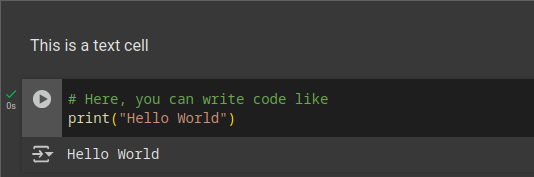
\includegraphics[width=0.7\textwidth]{logos/jupyter_notebook.png}

        \item Edit the notebooks in \textbf{Google Colab:}
            \url{https://colab.research.google.com/},
            
            more information in \texttt{student\_instructions.md} (ILIAS)
    \end{itemize}
\end{frame}

\begin{frame}{Overview: Exercises}
    \begin{itemize}
        \setlength\itemsep{1em}
        \item Notebooks are uploaded to ILIAS one week before the exercise
        \item Tutorial notebooks: read the text, click through the cells, try to
            understand the concepts and how the code works
        \item Exercise notebooks: apply the topics from the tutorial notebooks
            to a similar problem
        \item After the exercise: solution notebooks for the exercises are
            uploaded to ILIAS
        \item Questions: ask in the exercise, write in the ILIAS forum or mail
            at \url{leonie.pfeffer@kit.edu} or \url{maike.vogelbacher@kit.edu}
    \end{itemize}
\end{frame}

\begin{frame}{Dates}
    Every two weeks 12-3pm in the computer room (30.44, 4th floor):
    \begin{itemize}
        \setlength\itemsep{1em}
        \item 28.04. (today)
        \item 12.05.
        \item 26.05.
        \item \sout{09.06.} (holiday)
        \item 23.06.
        \item 07.07.
        \item 21.07.
    \end{itemize}
\end{frame}

\begin{frame}{Additional Resources}
    \begin{itemize}
        \setlength\itemsep{2em}
        \item bwGPT (alternative to ChatGPT): \url{https://bwgpt.scc.kit.edu/login?}

            $\Rightarrow$ log in with your KIT account
        \item Various forums, just search for your problem in your favorite
            search engine
        \item Numpy / Pandas / Sklearn documentation
            \vfill
            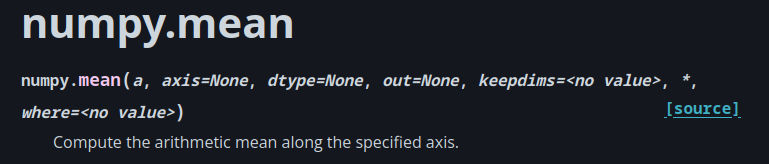
\includegraphics[width=0.7\textwidth]{./logos/numpy_doc.png}
    \end{itemize}
\end{frame}

\section{Today's Topics}
\begin{frame}{Today's Topics}
    \begin{itemize}
        \setlength\itemsep{2em}
        \item Python basics (\texttt{0.1\_Python\_Crashkurs.ipynb})
        \item Pandas tutorial and exercise
            (\texttt{1.1\_Pandas\_Crashcourse.ipynb} and
            \texttt{1.2\_Pandas\_Exercise.ipynb})
        \item Numpy tutorial (\texttt{2.1\_Numpy\_Crashcourse.ipynb})
    \end{itemize}
\end{frame}

\begin{frame}{Demonstration}
    \centering{Jupyter Notebook in Google Colab...}
    \vfill
    \centering{Summary: \texttt{student\_instructions.md}}
\end{frame}


\appendix
% Slides form here will not be counted in the page numbering nor will they
% appear in the navigation bar
\beginbackup

% \begin{frame}{Literature}
%     \printbibliography
% \end{frame}

\backupend
\end{document}
